\documentclass[11pt,dvipsnames]{article}
\usepackage{algorithm}
\usepackage{algpseudocode}
\usepackage{fullpage}
\usepackage[a3paper, landscape]{geometry}
\usepackage{graphicx}
\usepackage{amsmath}
\usepackage{amssymb}
\usepackage{verbatim}
\usepackage{xspace}
\usepackage{tikz}
%\usepackage[dvipsnames]{xcolor}

\usepackage{letltxmacro}
\makeatletter
\let\oldr@@t\r@@t
\def\r@@t#1#2{%
\setbox0=\hbox{$\oldr@@t#1{#2\,}$}\dimen0=\ht0
\advance\dimen0-0.2\ht0
\setbox2=\hbox{\vrule height\ht0 depth -\dimen0}%
{\box0\lower0.4pt\box2}}
\LetLtxMacro{\oldsqrt}{\sqrt}
\renewcommand*{\sqrt}[2][\ ]{\oldsqrt[#1]{#2}}
\makeatother

\DeclareMathOperator{\Tr}{Tr}

\newcommand{\ensuretext}[1]{#1}
\newcommand{\mycomment}[3]{\ensuretext{\textcolor{#3}{[#1 #2]}}}
\newcommand{\ammarker}{\ensuretext{\textcolor{red}{\ensuremath{^{\textsc{A}}_{\textsc{M}}}}}}
\newcommand{\am}[1]{\mycomment{\ammarker}{#1}{red}}
\begin{document}

\title{DiffusionModels}

\author{}

\maketitle

\section*{Introduction}

\begin{figure}
\resizebox{\textwidth}{!}{%
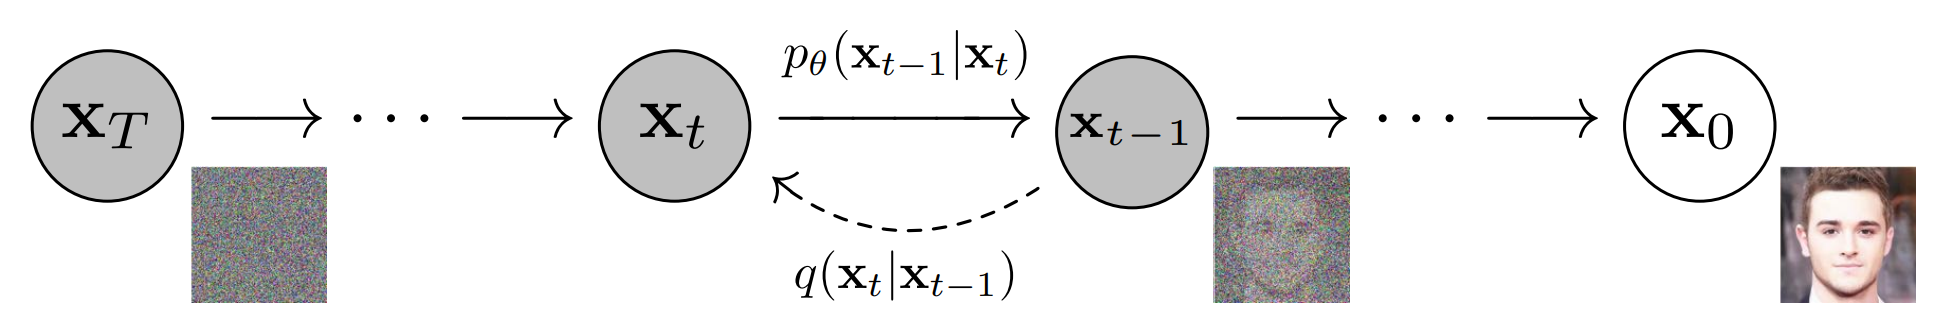
\includegraphics{model.png}
}
\caption{The model described here}
\label{fig:model}
\end{figure}

In this document I try to derive \emph{diffusion models}, which are a class of
generative models. The most common use case, and the one we will
focus on here is that of \emph{image} generation.

We will have two models, a \emph{forward} diffusion model that takes an image and
corrupts it slightly with Gaussian noise, and a \emph{reverse} diffusion model that
takes a noisy version of an image and attempts to remove the noise. These two models
will be applied multiple times to an image in order to turn a clean image into (nearly)
pure Gaussian noise, or to turn Gaussian noise into a clean image respectively.
We will call the clean image $x_0$ and the final most corrupted image, which is assumed
to be approximately pure Gaussian noise, $x_T$. See Figure~\ref{fig:model} for a graphical
representation of this process.

\section{Forward Model}
To take one step towards noisifying an image $x_t$, we would intuitively like to take
the previous image and add a small amount (call it $\beta$) of Gaussian noise. That is to say a first,
na\"ive approach would be to let $x_{t+1} = x_t + n$, where $n \sim \mathcal{N}(0, \beta)$.

It would be nice, however, if we could normalize our data such that $x_0$ has mean $0$
and variance $1$, and then maintain these nice properties throughout the process.
Recall that the mean of the sum of two random variables is just the sum of their means,
and similarly the variance of two random variables is just the sum of their variances.
That means, as defined, $\bar x_{t+1} = \bar x_t + \bar{n} = 0 + 0 = 0$ as desired, but
$\text{Var}(x_{t+1}) = \text{Var}(x_t) + \beta = 1 + \beta$.

To counteract this undesirable increase in variance we simply redefine $x_{t+1}$ as
$x_{t+1} = \sqrt{1 - \beta} \cdot x_t + n$. Since if $x$ is a random variable and $c$ is a
constant $\text{Var}(cx) = c^2\text{Var}(x)$, now
$\text{Var}(x_{t+1}) = (\sqrt{1 - \beta})^2\text{Var}(x) + \text{Var}(n) = (1 - \beta) + \beta = 1$,
as desired.

It is common to reparameterize such equations so that the noise component is directly drawn as
$\epsilon \sim \mathcal{N}(0, 1)$ to make computation easier, so we will take as our final form
$x_{t+1} = \sqrt{1 - \beta} \cdot x_t + \sqrt{\beta} \cdot \epsilon$.

In order to let our model be slightly more general, instead of taking $\beta$ to be a single constant,
we will let it change according to some fixed schedule and call each of these constants $\beta_t$.
In proper mathematical notation we may write $x_{t+1} \sim \mathcal{N}(\sqrt{1 - \beta_t} \cdot x_t, \beta_t^2)$.

\subsection{Direct Calculation of $x_t$ from $x_0$}
This model has another nice property in that $x_t$ can be easily computed from $x_0$ directly.
Let $\alpha_t = 1 - \beta_t$, $\bar\alpha_t = \prod_{i=1}^T \alpha_i$, and $\bar\beta_t = 1 - \bar\alpha_t$.
Then we have $x_t = \sqrt{1 - \bar\beta_t} \cdot x_{t-1} + \sqrt{\bar\beta_t} \cdot \epsilon$.

We can see this by induction. Notice that if $t=1$ then the above equation reads
$x_1 = \sqrt{1 - \bar\beta_t} \cdot x_{t-1} + \sqrt{\bar\beta_t} \cdot \epsilon$.
We can simplify
$\bar\beta_t = 1 - \bar\alpha_t = 1 - \prod_{i=1}^1 \alpha_i = 1 - \prod{i=1}^1 (1 - \beta_i) = 1 - (1 - \beta_1) = \beta_1$,
so our definition of $x_1$ reduces to $x_1 = \sqrt{1 - \beta_1} \cdot x_0 + \sqrt{\beta_1} \cdot \epsilon$, which we know
to be correct.

Now let us assume that $x_t = \sqrt{1 - \bar\beta_t} \cdot x_{t-1} + \sqrt{\bar\beta_t} \cdot \epsilon$.
We know from the one-step definition that $x_{t+1} = \sqrt{1 - \beta_{t+1}} \cdot \mathbin{\color{BrickRed}x_t} + \sqrt{\eta_{t+1}} \cdot \epsilon$.
Let us plug in the above definition of $x_t$:
\begin{equation*}
\begin{split}
x_{t+1} &= \sqrt{1 - \beta_{t+1}} \cdot (\mathbin{\color{BrickRed} \sqrt{1 - \bar\beta_t} \cdot x_{t-1} + \sqrt{\bar\beta_t} \cdot \epsilon_1}) + \sqrt{\beta_{t+1}} \cdot \epsilon_2 \\
& = \sqrt{\alpha_{t+1}} \cdot \left(\sqrt{\bar\alpha_t} \cdot x_{t-1} + \sqrt{1 - \bar\alpha_t} \cdot \epsilon_1\right) + \sqrt{1 - \alpha_{t+1}} \cdot \epsilon_2 \\
& = \sqrt{\alpha_{t+1}} \cdot \sqrt{\bar\alpha_t} \cdot x_{t-1} + \sqrt{\alpha_{t+1}} \cdot \sqrt{1 - \bar\alpha_t} \cdot \epsilon_1 + \sqrt{1 - \alpha_{t+1}} \cdot \epsilon_2 \\
& = \sqrt{\alpha_{t+1}} \cdot \sqrt{\bar\alpha_t} \cdot x_{t-1} + \sqrt{\alpha_{t+1} (1 - \bar\alpha_t) + (1 - \alpha_{t+1})} \cdot \epsilon_3 \\
& = \sqrt{\alpha_{t+1}} \cdot \sqrt{\bar\alpha_t} \cdot x_{t-1} + \sqrt{\alpha_{t+1} - \alpha_{t+1} \cdot \bar\alpha_t + 1 - \alpha_{t+1}} \cdot \epsilon_3 \\
& = \sqrt{\bar\alpha_{t+1}} \cdot x_{t-1} + \sqrt{1 - \bar\alpha_{t+1}} \cdot \epsilon_3 \\
& = \sqrt{1 - \bar\beta_{t+1}} \cdot x_{t-1} + \sqrt{\bar\beta_{t+1}} \cdot \epsilon_3
\end{split}
\end{equation*}

where the one confusing line comes from the fact that $c \cdot \epsilon_1 + d \cdot \epsilon_2 = \sqrt{c^2 + d^2} \epsilon_3$,
due to properties of the variance of the sum of two random variables. Thus, by induction, we have shown that this formula holds for all $t \in [1, T]$.

\subsection{Summary}
\label{sec:forwardsummary}
Here we give a summary of important equations from this section.
\begin{equation*}
\begin{split}
\beta_t & \text{is a small constant for $1 < t < T$} \\
\alpha_t & = 1 - \beta_t \\
\bar\alpha_t & = \prod_{i=1}^t \alpha_i \\
\bar\beta_t & = 1 - \bar\alpha_t \\
x_t & = \sqrt{1 - \beta_t} \cdot x_{t-1} + \sqrt{\beta_t} \cdot \epsilon \\
 & = \sqrt{1 - \bar\beta_t} \cdot x_0 + \sqrt{\bar\beta_t} \cdot \epsilon \\
\end{split}
\end{equation*}

\section{Reverse Model}
The reverse model attempts to remove noise from an image.
Like the forward model, it will also be Gaussian and also be applied over
a sequence of $T$ steps. 
Unlike the forward model, the reverse model will have its mean parameterized
by a neural network. In theory the per-dimension variance could also be learned
by a neural net, but we will follow the established literature in assuming that
the variance at time step $t$ is the same as it is in the forward model: $\beta_t \cdot I$.
This means according to our reverse model $x_{t - 1} \sim \mathcal{N}(\mu_\theta(x_t, t), \beta_t \cdot I)$.

\subsection{Summary}
Here we give a summary of important equations from this section.
\begin{equation*}
\begin{split}
x_{t-1} = \mu_\theta(x_t, t) + \sqrt{\beta_t} \cdot \epsilon \\
\end{split}
\end{equation*}

\section{Background}
In this section we will review a few key concepts that will play a role in the derivation of the loss function.
Note that in this section the symbols $p$ and $q$ here are meant to be general, and need not represent the same
functions or distributions notated with the same symbols in other sections of this document.

\subsection{KL Divergence}
Recall that the KL divergence is a non-symmetric way to measure the (dis)similarity between
two distributions. It will play a large role in our loss function so we will briefly review it
and some of its properties here.

The KL divergence between two distributions $p$ and $q$
is defined as $\text{KL}(p \mid\mid q) := \mathbb{E}_p \left[\log \frac{p(x)}{q(x)}\right]$, where the double bar
indicates that the function is non-symmetric in its arguments. We can use the definition
of the expectation operator rewrite this as $\text{KL}(p \mid\mid q) = \int_x p(x) \cdot \log \frac{p(x)}{q(x)} \,dx$.

While we will not prove them here, we will also mention two key properties of KL divergence that we will later use.
First, KL divergence is always non-negative. Second, KL divergence is minimized when $p(x) = q(x)$. In this case,
$\text{KL}(p \mid\mid q) = 0$.

\subsection{ELBO}
Here we will derive the \emph{ELBO}, or evidence lower bound.
In Baysian model land the quantity $\log p(x)$ is called the \emph{evidence}.
It measures the quality of the model by evaluating the probability it assigns to known data.
Our goal is to find a lower bound on the evidence, which we can then maximize.

\subsubsection{Derivation 1}
We begin with our goal $\log p(x)$. We will add a dependence on another random variable $z$, which
we then marginalize out: $\log p(x) = \log \int_z p(x, z) \, dz$. If we have another distribution $q(z)$
we can then write $\log \int_z p(x, z) \, dz = \log \int_z p(x, z) \frac{q(z)}{q(z)} \, dz$.
Rearranging then gives $\log \int_z q(z) \frac{p(x, z)}{q(z)} \, dz$.
By the definition of the expectation operator this equals $\log \mathbb{E}_q \left[ \frac{p(x, z)}{q(z)} \right]$.
Since $\log$ is a convex function, by Jensen's Inequality we can write
$\log \mathbb{E}_q \left[ \frac{p(x, z)}{q(z)} \right] \ge \mathbb{E}_q \left[ \log \frac{p(x, z)}{q(z)} \right]$.

In the end this leaves us with the following key equation:
$\log p(x) \ge \mathbb{E}_q \left[ \log \frac{p(x, z)}{q(z)} \right] = -\mathbb{E}_q \left[ \log \frac{q(z)}{p(x, z)} \right] = -\text{KL}(q(z) \mid\mid p(x, z))$.
The right hand side of this inequality is known as the ELBO.

\subsubsection{Derivation 2}
Another way of deriving this is to start by observing that since KL divergence is always non-negative
$\text{KL}(q(z) \mid\mid p(z \mid x)) \ge 0$ for all distributions $p$ and $q$.
\begin{equation*}
\begin{split}
0 &\le \text{KL}(q(z) \mid\mid p(z \mid x)) \\
& = \mathbb{E}_q \left[\log q(z) - \log p(z \mid x)\right] \\
& = \mathbb{E}_q \left[\log q(z) - \log \frac{p(x, z)}{p(x)} \right] \\
& = \mathbb{E}_q \left[\log q(z) - \log p(x, z) + \log p(x)\right] \\
& = \mathbb{E}_q \left[\log q(z) - \log p(x, z)\right] + \mathbb{E}_q \left[ \log p(x) \right]\\
& = \text{KL}(q(z) \mid\mid p(x, z)) + \log p(x) \\
\end{split}
\end{equation*}

We now have shown $0 \le \text{KL}(q(z) \mid\mid p(x, z)) + \log p(x)$, which implies $-\text{KL}(q(z) \mid\mid p(x, z)) \le \log p(x)$, as desired.

\section{Loss Function}
\subsection{Notation}
Let us notate the reverse model as $p_\theta$, writing
$p_\theta(x_{t-1} \mid x_t) = \mu_\theta(x_t, t) + \sqrt{\beta_t} \cdot \epsilon$.
As a notational shortcut we will write $p_\theta(x_{0:T}) = p(x_T) \prod_{t=1}^T p_\theta(x_{t-1} \mid x_t)$
to represent the probability of generating $x_0$ from $x_T$, multiplying the probabilities of all $T$
individual steps.

Similarly we will notate the forward model as $q$. While we could simply write
$q(x_t \mid x_{t-1})$, for reasons we will see later, we will also condition on $x_0$:
$q(x_t \mid x_{t-1}, x_0)$. This extra conditioning affords us the flexibility to interchangeably use
the two definitions we have for the forward model of $x_t$:
\begin{equation*}
\begin{split}
q(x_t \mid x_{t-1}, x_0) &= \sqrt{1 - \beta_t} \cdot x_{t-1} + \sqrt{\beta_t} \cdot \epsilon \\
&= \sqrt{1 - \bar\beta_t} \cdot x_0 + \sqrt{\bar\beta_t} \cdot \epsilon
\end{split}
\end{equation*}
Again, similar to the reverse model, we will write $q(x_1:T \mid x_0) = \prod_{t=1}^T q(x_t \mid x_{t-1}, x_0)$
to compactly represent the probability of generating $x_T$ from $x_0$ over all $T$ steps.

\subsection{Deriving the three-part loss}
\label{sec:threepartloss}
We would like to maximize the evidence of our model $p(x_0)$, or equivalently minimize the
opposite of the log probability $-\log p(x_0)$.
We can use the ELBO inequality and take $z = x_{1:T}$ to write
$-\log p(x_0) \le -KL(q(x_{1:T} \mid x_0) \mid\mid p(x_{0:T}))$.
This expression, after a bunch more simplification, will be the loss function we use to train
the neural network.

Let us use the definition of KL divergence, along with the definitions of $q(x_{1:T} \mid x_0)$
and $p(x_{0:T})$ to write
\begin{equation*}
\begin{split}
\mathcal{L} &= -KL(q(x_{1:T} \mid x_0) \mid\mid p(x_{0:T})) \\
&= \mathbb{E}_q \left[\log \prod_{t=1}^T q(x_t \mid x_{t-1}, x_0) - \log \left( p(x_T) \prod_{t=1}^T p(x_{t-1} \mid x_t) \right) \right] \\
&= -\log p(x_T) + \mathbb{E}_q \left[\sum_{t=1}^T \log q(x_t \mid x_{t-1}, x_0) - \sum_{t=1}^T \log p(x_{t-1} \mid x_t) \right] \\
&= -\log p(x_T) + \mathbb{E}_q \left[\log q(x_1 \mid x_0) + \mathbin{\color{BrickRed}\sum_{t=2}^T \log q(x_t \mid x_{t-1}, x_0)} - \sum_{t=2}^T \log p(x_{t-1} \mid x_t) - \log p(x_0 \mid x_1) \right] \\
\end{split}
\end{equation*}

Let's zoom in a bit on the term in red. Using Bayes' Rule and then simplifying we get:
\begin{equation*}
\begin{split}
& \sum_{t=2}^T \log q(x_t \mid x_{t-1}, x_0) \\
& = \sum_{t=2}^T \log q(x_{t-1} \mid x_t, x_0) \cdot \frac{q(x_t \mid x_0)}{q(x_{t-1} \mid x_0)} \\
& = \sum_{t=2}^T \log q(x_{t-1} \mid x_t, x_0) + \sum_{t=2}^T \log q(x_t \mid x_0) - \sum_{t=2}^T \log q(x_{t-1} \mid x_0) \\
& = \sum_{t=2}^T \log q(x_{t-1} \mid x_t, x_0) + \log q(x_T \mid x_0) + \sum_{t=2}^{T-1} \log q(x_t \mid x_0) - \sum_{t=3}^T \log q(x_{t-1} \mid x_0) - \log q(x_1 \mid x_0) \\
& = \sum_{t=2}^T \log q(x_{t-1} \mid x_t, x_0) + \log q(x_T \mid x_0) + \sum_{t=2}^{T-1} \log q(x_t \mid x_0) - \sum_{t=2}^{T-1} \log q(x_t \mid x_0) - \log q(x_1 \mid x_0) \\
& = \sum_{t=2}^T \log q(x_{t-1} \mid x_t, x_0) + \log q(x_T \mid x_0) - \log q(x_1 \mid x_0) \\
\end{split}
\end{equation*}

Plugging this final expression back in for the red piece gives us:
\begin{equation*}
\begin{split}
\mathcal{L} &= -\log p(x_T) + \mathbb{E}_q \left[\sum_{t=2}^T \log q(x_{t-1} \mid x_t, x_0) + \log q(x_T \mid x_0) - \sum_{t=2}^T \log p(x_{t-1} \mid x_t) - \log p(x_0 \mid x_1) \right] \\
&= \mathbb{E}_q \left[ \log q(x_T \mid x_0) - \log p(x_T) + \sum_{t=2}^T \big( \log q(x_{t-1} \mid x_t, x_0) - \log p(x_{t-1} \mid x_t) \big) - \log p(x_0 \mid x_1) \right] \\
&= \mathbb{E}_q \left[ \text{KL}(q(x_T \mid x_0) \mid\mid p(x_T)) + \sum_{t=2}^T \text{KL}(q(x_{t-1} \mid x_t, x_0) \mid\mid p(x_{t-1} \mid x_t)) - \log p(x_0 \mid x_1) \right] \\
\end{split}
\end{equation*}


Notice that we now have a single term of this loss function for each $t \in [0, T]$:
\begin{equation*}
\begin{split}
\mathcal{L} &= \mathbb{E}_q \left[ \sum_{t=0}^T \mathcal{L}_t \right] \; \text{where} \\
\mathcal{L}_0 &= -\log p(x_0 \mid x_1) \\
\mathcal{L}_t &= \text{KL}(q(x_{t-1} \mid x_t, x_0) \mid\mid p(x_{t-1} \mid x_{t})) \; \text{for} \; t \in [1, T-1] \\
\mathcal{L}_T &= \text{KL}(q(x_T \mid x_0) \mid\mid p(x_T)) \\
\end{split}
\end{equation*}

Next we will discuss each of these terms in turn, and find a tractable expression for each that we can use to compute
our neural network's loss function.

\subsection{$\mathcal{L}_0$}
First up is $\mathcal{L}_0 = -\log p(x_0 \mid x_1)$.
$p$ is a normal Gaussian with mean $\mu_\theta(x_1)$ being our neural network's output on $x_1$ and variance $\beta_1$.
This means

\begin{equation*}
\begin{split}
-\log p(x_0 \mid x_1) &= \frac{1}{2} \log\det(2\pi\beta_1 I) +-\frac{1}{2}(x_0 - \mu_\theta(x_1))^T(\beta_1I)^{-1}(x_0 - \mu_\theta(x_1)) \\
&= \frac{D}{2} \log (2\pi\beta_1) + \frac{1}{2\beta_1} \lVert x_0 - \mu_\theta(x_1) \rVert^2 \\
&= \frac{1}{2\beta_1} \lVert x_0 - \mu_\theta(x_1) \rVert^2 + C \\
\end{split}
\end{equation*}

where $C$ is some constant that does not depend on the parameters of our neural network, and as such can be ommited from our loss function.

\subsection{$\mathcal{L}_t$ for $1 \leq t \leq T - 1$}
Next we turn our attention to $\mathcal{L}_t$ for $1 \le t \le T - 1$, which is the KL divergence between two distributions.
We have a good understanding of $p(x_{t-1} \mid x_t) \sim \mathcal{N}(\mu_\theta(x_t), \beta_tI)$.
This is just a normal distribution with its mean computed by our neural network when given the input $x_t$.
The other distribution in question, $q(x_{t-1} \mid x_t, x_0)$, is a bit tougher to compute. It is the \emph{inverse} of the
distribution $q(x_t \mid x_{t-1}, x_0)$, achieved by applying Bayes' rule in \S\ref{sec:threepartloss}.

To find a tractable form of $q(x_{t-1} \ mid x_t, x_0)$ we will again use Bayes' rule to write
\begin{equation*}
q(x_{t-1} \mid x_t, x_0) = q(x_t \mid x_{t-1}, x_0) \cdot \frac{q(x_{t-1} \mid x_0)}{q(x_t \mid x_0)}
\end{equation*}

We will rewrite each of these three pieces using the definitions of $q$ from \S\ref{sec:forwardsummary}
\am{the referenced section never gives the Normal definition of these things}:
\begin{equation*}
\begin{split}
q(x_t \mid x_{t-1}, x_0) & \sim \mathcal{N}\left(\sqrt{1 - \beta_t} \, x_{t-1}, \beta_t I \right) \\
q(x_{t-1} \mid x_0) & \sim \mathcal{N}\left(\sqrt{1 - \bar\beta_{t-1}} \, x_0, \bar\beta_{t-1} I \right) \\
q(x_t \mid x_0) & \sim \mathcal{N}\left(\sqrt{1 - \bar\beta_t} \, x_0, \bar\beta_t I \right) \\
\mathcal{N} \left( \mu, \Sigma \right) &= \det(2\pi\Sigma)^{-\frac{1}{2}} \cdot e^{-\frac{1}{2}(x - \mu)^T \Sigma^{-1} (x - \mu)} \\
\end{split}
\end{equation*}

Sadly, there's no shortcut to the math. We have to just smash all these together, do a bunch of algebra, and see what shakes out.
It is, however, slightly cleaner in log space, so we will start with $\log q(x_{t-1} \mid x_t, x_0)$ and then re-exponentiate at the end.

\begin{equation*}
\begin{split}
\log q(x_{t-1} \mid x_t, x_0) &= \log \left( q(x_t \mid x_{t-1}, x_0) \cdot \frac{q(x_{t-1} \mid x_0)}{q(x_t \mid x_0)} \right) \\
&= \log q(x_t \mid x_{t-1}, x_0) + \log q(x_{t-1} \mid x_0) - \log q(x_t \mid x_0) \\
&= \log \left(\det(2\pi\beta_tI)^{-\frac{1}{2}} \cdot e^{-\frac{1}{2} \left(x_t - \sqrt{1 - \beta_t} \, x_{t-1}\right)^T \left(\beta_t I\right)^{-1} \left(x_t - \sqrt{1 - \beta_t} \, x_{t-1}\right)} \right)
+ \log \left(\det(2\pi\bar\beta_{t-1}I)^{-\frac{1}{2}} \cdot e^{-\frac{1}{2} \left(x_{t-1} - \sqrt{1 - \bar\beta_{t-1}} \, x_0\right)^T \left(\bar\beta_{t-1}I\right)^{-1} \left(x_{t-1} - \sqrt{1 - \bar\beta_{t-1}} \, x_0 \right)} \right)
- \log \left( \det(2\pi\bar\beta_tI)^{-\frac{1}{2}} \cdot e^{-\frac{1}{2} \left(x_t - \sqrt{1 - \bar\beta_t} \, x_0 \right)^T \left(\bar\beta_t I \right)^{-1} \left(x_t - \sqrt{1 - \bar\beta_t} x_0 \right)} \right) \\
\end{split}
\end{equation*}

Pretty heinous looking, right? Thankfully since our variance matrices are all of the form $c I$, their determinants and inverses are very easy to work out.
Recall that $\det(c A) = c^D \det(A)$, $\det(I) = 1$, and $\left(c I\right)^{-1} = \frac{1}{c}I$, where $D$ is the dimensionality of matrix $A$ (and thus of the data we're working with). Thus $\det(2 \pi \beta I) = (2 \pi \beta)^D$.

Since matrix multiplication by a constant is commutative, we can also rewrite
\begin {equation*}
\begin{split}
(x - \mu)^T (\beta I)^{-1} (x - \mu) &= (x - \mu)^T \left(\frac{1}{\beta} I \right) (x - \mu) \\
&= \frac{1}{\beta} (x - \mu)^T I (x - \mu) \\
&= \frac{1}{\beta} (x - \mu)^T (x - \mu) \\
&= \frac{1}{\beta} \lVert x - \mu \rVert^2 \\
\end{split}
\end{equation*}

Plugging these simplications into what we had from above we get
\begin{equation*}
\begin{split}
\log q(x_{t-1} \mid x_t, x_0) &= \log \left( (2 \pi \beta_t)^{-\frac{D}{2}} \cdot e^{-\frac{1}{2\beta_t} \lVert x_t - \sqrt{1 - \beta_t} x_{t-1} \rVert^2} \right)
+ \log \left( (2 \pi \bar\beta_{t-1})^{-\frac{D}{2}} e^{-\frac{1}{2\bar\beta_{t-1}} \lVert x_{t-1} - \sqrt{1 - \bar\beta_{t-1}} x_0 \rVert^2} \right)
- \log \left( (2 \pi \bar\beta_t)^{-\frac{D}{2}} e^{-\frac{1}{2\bar\beta_t} \lVert x_t - \sqrt{1 - \bar\beta_t} x_0 \rVert^2} \right) \\
&= -\frac{D}{2}\log(2\pi\beta_t) - \frac{D}{2} \log(2\pi\bar\beta_{t-1}) + \frac{D}{2} \log(2\pi\bar\beta_t) 
-\frac{1}{2\beta_t} \lVert x_t - \sqrt{1 - \beta_t} \, x_{t-1} \rVert^2 \\
&-\frac{1}{2\bar\beta_{t-1}} \lVert x_{t-1} - \sqrt{1 - \bar\beta_{t-1}} \, x_0 \rVert^2
+\frac{1}{2\bar\beta_t} \lVert x_t - \sqrt{1 - \bar\beta_t} \, x_0 \rVert^2 \\
&= -\frac{D}{2}\log\left(\frac{(2\pi\beta_t) (2\pi\bar\beta_{t-1})}{2\pi\bar\beta_t}\right)
-\frac{1}{2\beta_t} \sum_{i=1}^D \left(x_{t,i}^2 - 2\sqrt{1 - \beta_t} \, x_{t-1,i} x_{t, i} + (1 - \beta_t)x_{t-1, i}^2 \right)
-\frac{1}{2\bar\beta_{t-1}} \sum_{i=1}^D \left( x_{t-1,i}^2 - 2 \sqrt{1 - \bar\beta_{t-1}} \, x_{0, i} x_{t-1, i} + (1 - \bar\beta_{t-1}) x_{0,i}^2 \right)
+\frac{1}{2\bar\beta_t} \sum_{i=1}^D \left( x_{t,i}^2 - 2\sqrt{1 - \bar\beta_t} \, x_{0,i} x_{t, i} + (1 - \bar\beta_t)x_{0,i}^2 \right)\\
&= -\frac{D}{2}\log\left(\frac{2\pi\beta_t\bar\beta_{t-1}}{\bar\beta_t}\right)
\sum_{i=1}^D \bigg( -\frac{1}{2\beta_t} x_{t,i}^2 + \frac{\sqrt{1 - \beta_t}}{\beta_t} x_{t-1,i} x_{t, i} -\frac{1 - \beta_t}{2\beta_t} x_{t-1,i}^2
-\frac{1}{2\bar\beta_{t-1}} x_{t-1,i}^2 + \frac{\sqrt{1 - \bar\beta_{t-1}}}{\bar\beta_{t-1}} x_{0, i} x_{t-1, i} - \frac{1 - \bar\beta_{t-1}}{2\bar\beta_{t-1}} x_{0,i}^2
+\frac{1}{2\bar\beta_t} x_{t,i}^2 - \frac{2\sqrt{1 - \bar\beta_t}}{2\bar\beta_t} x_{0,i} x_{t, i} + \frac{1 - \bar\beta_t}{2\bar\beta_t}x_{0,i}^2 \bigg) \\
&= -\frac{D}{2}\log\left(\frac{2\pi\beta_t\bar\beta_{t-1}}{\bar\beta_t}\right)
+\sum_{i=1}^D \Bigg( \left(-\frac{1 - \beta_t}{2\beta_t} - \frac{1}{2\bar\beta_{t-1}} \right) x_{t-1,i}^2
+ \left( \frac{\sqrt{1 - \beta_t}}{\beta_t} x_{t, i} + \frac{\sqrt{1 - \bar\beta_{t-1}}}{\bar\beta_{t-1}} x_{0, i} \right) x_{t-1, i}
+ \left( -\frac{1}{2\beta_t} x_{t,i}^2 - \frac{1 - \bar\beta_{t-1}}{2\bar\beta_{t-1}} x_{0,i}^2 +\frac{1}{2\bar\beta_t} x_{t,i}^2 - \frac{2\sqrt{1 - \bar\beta_t}}{2\bar\beta_t} x_{0,i} x_{t, i} + \frac{1 - \bar\beta_t}{2\bar\beta_t}x_{0,i}^2 \right) \Bigg) \\
%
&= -\frac{D}{2}\log\left(\frac{2\pi\beta_t\bar\beta_{t-1}}{\bar\beta_t}\right)
-\frac{1}{2} \sum_{i=1}^D \Bigg( \frac{\bar\beta_t}{\beta_t\bar\beta_{t-1}} x_{t-1,i}^2
- \left( \frac{2 \bar\beta_t}{\bar\beta_{t-1}\beta_t} \left(\frac{\bar\beta_{t-1}\sqrt{1 - \beta_t}}{\bar\beta_t} x_{t, i} + \frac{\beta_t\sqrt{1 - \bar\beta_{t-1}}}{\bar\beta_t} x_{0, i} \right) \right) x_{t-1, i}
- \left( \left( \frac{1}{\bar\beta_t} - \frac{1}{\beta_t} \right) x_{t,i}^2 - \frac{2\sqrt{1 - \bar\beta_t}}{\bar\beta_t} x_{0,i} x_{t, i} + \left( \frac{1 - \bar\beta_t}{\bar\beta_t} - \frac{1 - \bar\beta_{t-1}}{\bar\beta_{t-1}} \right) x_{0,i}^2 \right) \Bigg) \\
\end{split}
\end{equation*}

Now let us focus for a moment on the last term, the one that does not depend on $x_{t-1,i}$:
\begin{equation*}
\left( \frac{1}{\bar\beta_t} - \frac{1}{\beta_t} \right) x_{t,i}^2 - \frac{2\sqrt{1 - \bar\beta_t}}{\bar\beta_t} x_{0,i} x_{t, i} + \left( \frac{1 - \bar\beta_t}{\bar\beta_t} - \frac{1 - \bar\beta_{t-1}}{\bar\beta_{t-1}} \right) x_{0,i}^2 
\end{equation*}

The $x_{t,i}^2$ coefficient can be rewritten as
\begin{equation*}
\begin{split}
\frac{1}{\bar\beta_t} - \frac{1}{\beta_t} &= \frac{\beta_t - \bar\beta_t}{\bar\beta_t\beta_t} \\
&= \frac{(1 - \alpha_t) - (1 - \bar\alpha_t)} {\bar\beta_t\beta_t} \\
&= \frac{\bar\alpha_t - \alpha_t}{\bar\beta_t\beta_t} \\
&= \frac{\alpha_t (\bar\alpha_{t-1} - 1)}{\bar\beta_t\beta_t} \\
&= \frac{-\alpha_t\bar\beta_{t-1}}{\bar\beta_t\beta_t} \\
&= \frac{-\bar\beta_t}{\beta_t \bar\beta_{t-1}} \cdot \frac{\bar\beta_{t-1}^2 (1 - \beta_t)}{\bar\beta_t^2} \\
&= \frac{-\bar\beta_t}{\beta_t\bar\beta_{t-1}} \cdot \left( \frac{\beta_t \sqrt{1 - \bar\beta_{t-1}}}{\bar\beta_t} \right)^2
\end{split}
\end{equation*}

The $x_{0,i}^2$ coefficient can be rewritten as
\begin{equation*}
\begin{split}
\frac{1 - \bar\beta_t}{\bar\beta_t} - \frac{1 - \bar\beta_{t-1}}{\bar\beta_{t-1}} &= \left(\frac{1}{\bar\beta_t} - 1\right) - \left(\frac{1}{\bar\beta_{t-1}} - 1 \right) \\
&= \frac{1}{\bar\beta_t} - \frac{1}{\bar\beta_{t-1}} \\
&= \frac{\bar\beta_{t-1} - \bar\beta_t}{\bar\beta_t\bar\beta_{t-1}} \\
&= \frac{(1 - \bar\alpha_{t-1}) - (1 - \bar\alpha_t)}{\bar\beta_t\bar\beta_{t-1}} \\
&= \frac{\alpha_t\bar\alpha_{t-1} - \bar\alpha_{t-1}}{\bar\beta_t \bar\beta_{t-1}} \\
&= \frac{\bar\alpha_{t-1} (\alpha_t - 1)}{\bar\beta_t \bar\beta_{t-1}} \\
&= \frac{-\beta_t (1 - \beta_{t-1})}{\bar\beta_t \bar\beta_{t-1}} \\
&= \frac{-\bar\beta_t}{\beta_t\bar\beta_{t-1}} \cdot \frac{\beta_t^2 (1 - \bar\beta_{t-1})}{\bar\beta_t^2} \\
&= \frac{-\bar\beta_t}{\beta_t\bar\beta_{t-1}} \cdot \left( \frac{\beta_t \sqrt{1 - \bar\beta_{t-1}}}{\bar\beta_t} \right)^2
\end{split}
\end{equation*}

Next we take a brief interlude to note that
\begin{equation*}
\begin{split}
1 - \bar\beta_t &= \bar\alpha_t \\
&= \alpha_t \bar\alpha_{t-1} \\
&= (1 - \beta_t)(1 - \bar\beta_{t-1})
\end{split}
\end{equation*}

Finally we rewrite the cross term coefficient of $x_{0,i} x_{t, i}$ as
\begin{equation*}
\begin{split}
- \frac{2\sqrt{1 - \bar\beta_t}}{\bar\beta_t} &= \frac{-2\bar\beta_t}{\beta_t\bar\beta_{t-1}} \cdot \frac{\beta_t \bar\beta_{t-1}}{\bar\beta_t^2} \sqrt{1 - \bar\beta_t} \\
&=  \frac{-\bar\beta_t}{\beta_t\bar\beta_{t-1}} \cdot \frac{2\beta_t \bar\beta_{t-1}}{\bar\beta_t^2} \sqrt{1 - \beta_t} \sqrt{1 - \bar\beta_{t-1}} \\
&= \frac{-\bar\beta_t}{\beta_t\bar\beta_{t-1}} \cdot 2 \cdot \frac{\bar\beta_{t-1}\sqrt{1 - \beta_t}}{\bar\beta_t} \cdot \frac{\beta_t\sqrt{1 - \bar\beta_{t-1}}}{\bar\beta_t}
\end{split}
\end{equation*}

Putting all this together lets us rewrite the last term of our absolute unit of an expression for
$\log q(x_{t-1} \mid x_t, x_0)$ with

\begin{equation*}
\frac{-\bar\beta_t}{\beta_t\bar\beta_{t-1}} \left( \left( \frac{\beta_t\sqrt{1 - \bar\beta_{t-1}}}{\bar\beta_t} \right)^2 x_{t,i}^2
+ 2 \cdot \frac{\bar\beta_{t-1}\sqrt{1 - \beta_t}}{\bar\beta_t} \frac{\beta_t\sqrt{1 - \bar\beta_{t-1}}}{\bar\beta_t} x_{0, i} x_{t, i}
+ \left( \frac{\beta_t\sqrt{1 - \bar\beta_{t-1}}}{\bar\beta_t} \right)^2 x_{0,i}^2 \right)
\end{equation*}

Now plugging \emph{this} expression back into the whole monster we end up with
\begin{equation*}
\begin{split}
&\log q(x_{t-1} \mid x_t, x_0) \\
&= -\frac{D}{2}\log\left(\frac{2\pi\beta_t\bar\beta_{t-1}}{\bar\beta_t}\right)
-\frac{\bar\beta_t}{2\beta_t\bar\beta_{t-1}} \sum_{i=1}^D \Bigg( x_{t-1,i}^2 \\
&- 2 \left(\frac{\bar\beta_{t-1}\sqrt{1 - \beta_t}}{\bar\beta_t} x_{t, i} + \frac{\beta_t\sqrt{1 - \bar\beta_{t-1}}}{\bar\beta_t} x_{0, i} \right) x_{t-1, i} \\
&- \left( \left( \frac{\beta_t\sqrt{1 - \bar\beta_{t-1}}}{\bar\beta_t} \right)^2 x_{t,i}^2 
+ 2 \cdot \frac{\bar\beta_{t-1}\sqrt{1 - \beta_t}}{\bar\beta_t} \cdot \frac{\beta_t\sqrt{1 - \bar\beta_{t-1}}}{\bar\beta_t} x_{0, i} x_{t, i}
+ \left( \frac{\beta_t\sqrt{1 - \bar\beta_{t-1}}}{\bar\beta_t} \right)^2 x_{0,i}^2 \right) \\
&= -\frac{D}{2}\log\left(\frac{2\pi\beta_t\bar\beta_{t-1}}{\bar\beta_t}\right)
-\frac{\bar\beta_t}{2\beta_t\bar\beta_{t-1}} \sum_{i=1}^D \left( x_{t-1,i} -  \left(\frac{\bar\beta_{t-1}\sqrt{1 - \beta_t}}{\bar\beta_t} x_{t, i} + \frac{\beta_t\sqrt{1 - \bar\beta_{t-1}}}{\bar\beta_t} x_{0, i} \right) \right)^2
\end{split}
\end{equation*}

Now we can observe that if we let $\tilde\Sigma_t = \frac{\beta_t\bar\beta_{t-1}}{\bar\beta_t}$ and
$\tilde\mu_t = \frac{\bar\beta_{t-1}\sqrt{1 - \beta_t}}{\bar\beta_t} x_{t, i} + \frac{\beta_t\sqrt{1 - \bar\beta_{t-1}}}{\bar\beta_t} x_{0, i}$
then we have the very elegant result that $q(x_{t-1} \mid x_t, x_0) \sim \mathcal{N}(\tilde\mu_t, \tilde\Sigma_t I)$.

\subsubsection{KL Divergence between Gaussians}
This makes the quantity we actually want to compute, $\mathcal{L}_t = \text{KL}\left(q(x_{t-1} \mid x_t, x_0) \mid\mid p(x_{t-1} \mid x_t) \right)$ simply the
KL divergence between two Gaussians, which is easily computable in closed form.

\begin{equation*}
\begin{split}
&\text{KL}(\mathcal{N}(\mu_1, \Sigma_1) \mid\mid \mathcal{N}(\mu_2, \Sigma_2) \\
&= \mathbb{E}_{\mathcal{N}_1} \left[ \log \mathcal{N}(\mu_1, \Sigma_1) - \log \mathcal{N}(\mu_2, \Sigma_2) \right] \\
&= \mathbb{E}_{\mathcal{N}_1} \left[ \log(2\pi\det\Sigma_1)^{-\frac{1}{2}} - \frac{1}{2}(x - \mu_1)^T\Sigma_1^{-1}(x - \mu_1) - \log(2\pi\det\Sigma_2)^{-\frac{1}{2}} + \frac{1}{2}(x - \mu_2)^T\Sigma_2^{-1}(x - \mu_2) \right] \\
&= \frac{1}{2} \mathbb{E}_{\mathcal{N}_1} \left[ \log(2\pi\det\Sigma_2) - \log(2\pi\det\Sigma_1) + (x - \mu_2)^T\Sigma_2^{-1}(x - \mu_2) - (x - \mu_1)^T\Sigma_1^{-1}(x - \mu_1) \right] \\
\end{split}
\end{equation*}

We will now use equation 380 from \S8.2.2 of The Matrix Cookbook \footnote{https://www.math.uwaterloo.ca/~hwolkowi/matrixcookbook.pdf} which states that
$\mathbb{E}_{\mathcal{\mu, \Sigma}} \left[ (x - c)^T A (x - c) \right] = (\mu - c)^T A (\mu - c) + \Tr(\Sigma A)$ to continue simplifying.

\begin{equation*}
\begin{split}
&= \frac{1}{2} \left( \log \frac{\det\Sigma_2}{\det\Sigma_1} + (\mu_1 - \mu_2)^T\Sigma_2^{-1}(\mu_1 - \mu_2) + \Tr(\Sigma_1\Sigma_2^{-1}) - (\mu_1 - \mu_1)^T\Sigma_1^{-1}(\mu_1 - \mu_1) - \Tr(\Sigma_1\Sigma_1^{-1}) \right) \\
&= \frac{1}{2} \left( \log \frac{\det\Sigma_2}{\det\Sigma_1} + (\mu_1 - \mu_2)^T\Sigma_2^{-1}(\mu_1 - \mu_2) + \Tr(\Sigma_1\Sigma_2^{-1}) - D \right) \\
\end{split}
\end{equation*}

If we have variances of the forms $\Sigma_1 = \alpha I$ and $\Sigma_2 = \beta I$ then we can further simplify.
\begin{equation*}
\begin{split}
&= \frac{1}{2} \left( \log \frac{\alpha^D}{\beta^D} + \frac{1}{\beta}(\mu_1 - \mu_2)^T (\mu_1 - \mu_2) + \Tr(\frac{\alpha}{\beta}I) - D \right) \\
&= \frac{1}{2} \left( D \log \frac{\alpha}{\beta} + \frac{1}{\beta} \lVert \mu_1 - \mu_2 \rVert^2 + \frac{D\alpha}{\beta} - D \right) \\
&= \frac{D}{2} \left( \log \frac{\alpha}{\beta} + \frac{1}{D\beta} \lVert \mu_1 - \mu_2 \rVert^2 + \frac{\alpha}{\beta} - 1 \right) \\
\end{split}
\end{equation*}

Finally we can plug in our known distributions:
\begin{equation*}
\begin{split}
\mathcal{L}_t &= \text{KL} \left( q(x_{t-1} \mid x_t, x_0) \mid\mid p(x_{t-1} \mid x_t) \right) \\
&= \text{KL}\left( \mathcal{N} \left(\tilde\mu_t, \tilde\Sigma_t I \right) \mid\mid \mathcal{N} \left( \mu_\theta(x_t), \beta_t I \right) \right) \\
&= \frac{D}{2} \left( \log \frac{\tilde\Sigma_t}{\beta_t} + \frac{1}{D\beta_t} \lVert \tilde\mu_t - \mu_\theta(x_t) \rVert^2 + \frac{\tilde\Sigma_t}{\beta_t} - 1 \right) \\
&= \frac{1}{2\beta_t} \lVert \tilde\mu_t - \mu_\theta(x_t) \rVert^2 + C
\end{split}
\end{equation*}

where $C$ is a bunch of stuff that does not depend on $\theta$, the parameters of our neural network.


\subsection{$\mathcal{L}_T$}
Finally, we come to the easiest of the three terms, $\mathcal{T} = \text{KL}(q(x_t \mid x_0) \mid\mid p(x_T))$.
Recall that once we've chosen the constants $\beta_t$, $q$ is a deterministic Gaussian model and has nothing to
do with the neural network. Additionally, $x_T$ is the \emph{input} to our denoising neural network and is
assumed to be pure Gaussian noise. As such, the parameters of our neural network have no effect on either of the
two quantities being compared here, and $\text{KL}(q(x_t \mid x_0) \mid\mid p(x_T))$ is just some constant hanging
off the end of our loss function. Since it does not depend on our parameters at all, there will be no effect on our
backprop procedure if we simply drop this term outright. It doesn't get any easier than that!

\section{All together}
In total this means
\begin{equation*}
\begin{split}
\mathcal{L} &= \mathcal{L}_0 + \sum_{t=1}^{T} \mathcal{L}_t \\
&= \frac{1}{2\beta_1} \lVert x_0 - \mu_\theta(x_1) \rVert^2 + \sum_{t=2}^{T-1} \frac{1}{2\beta_t} \lVert \tilde\mu_t - \mu_\theta(x_t) \rVert^2 \\
\end{split}
\end{equation*}
where $\tilde\mu_t = \frac{\bar\beta_{t-1}\sqrt{1 - \beta_t}}{\bar\beta_t} x_{t, i} + \frac{\beta_t\sqrt{1 - \bar\beta_{t-1}}}{\bar\beta_t} x_{0, i}$

We can simplify this even further if we simply define $\bar\beta_t = 0$. Then the whole expression reduces to just
\begin{equation*}
\mathcal{L} = \sum_{t=1}^{T} \frac{1}{2\beta_t} \lVert \tilde\mu_t - \mu_\theta(x_t) \rVert^2
\end{equation*}

\section{Improvements}
\subsection{Predicting Noise}
We have determined that our loss can be written as
\begin{equation*}
\mathcal{L} = \sum_{t=1}^{T} \frac{1}{2\beta_t} \lVert \tilde\mu_t(x_t, x_0) - \mu_\theta(x_t) \rVert^2
\end{equation*}

but we also know that $x_t = \sqrt{1 - \bar\beta_t} x_0 + \sqrt{\bar\beta_t} \epsilon$, or equivalently
$x_0 = \frac{x_t - \sqrt{\bar\beta_t}\epsilon}{\sqrt{1 - \bar\beta_t}}$. We can plug this expression
for $x_0$ into the definition of $\tilde\mu_t(x_t, x_0)$ to find

\begin{equation*}
\begin{split}
\tilde\mu_t(x_t, x_0) &= \frac{\bar\beta_{t-1}\sqrt{1 - \beta_t}}{\bar\beta_t} x_t + \frac{\beta_t\sqrt{1 - \bar\beta_{t-1}}}{\bar\beta_t} x_0 \\
&= \frac{\bar\beta_{t-1}\sqrt{1 - \beta_t}}{\bar\beta_t} x_t + \frac{\beta_t\sqrt{1 - \bar\beta_{t-1}}}{\bar\beta_t} \cdot \frac{x_t - \sqrt{\bar\beta_t} \epsilon}{\sqrt{1 - \bar\beta_t}} \\
&= \left( \frac{\bar\beta_{t-1}\sqrt{1 - \beta_t}}{\bar\beta_t} + \frac{\beta_t\sqrt{1 - \bar\beta_{t-1}}}{\bar\beta_t\sqrt{1 - \bar\beta_t}} \right) x_t - \frac{\beta_t\sqrt{1 - \bar\beta_{t-1}}\sqrt{\bar\beta_t}}{\bar\beta_t\sqrt{1 - \bar\beta_t}} \epsilon \\
&= \left( \frac{\sqrt{1 - \bar\beta_t} \bar\beta_{t-1}\sqrt{1 - \beta_t} + \beta_t\sqrt{1 - \bar\beta_{t-1}}}{\bar\beta_t\sqrt{1 - \bar\beta_t}} \right) x_t - \frac{\beta_t\sqrt{1 - \bar\beta_{t-1}}\sqrt{\bar\beta_t}}{\bar\beta_t\sqrt{1 - \bar\beta_t}} \epsilon \\
&= \left( \frac{\sqrt{\bar\alpha_t} (1 - \bar\alpha_{t-1}) \sqrt{\alpha_t} + (1 - \alpha_t) \sqrt{\bar\alpha_{t-1}}}{(1 - \bar\alpha_t) \sqrt{\bar\alpha_t}} \right) x_t - \frac{(1 - \alpha_t) \sqrt{\bar\alpha_{t-1}} \sqrt{1 - \bar\alpha_t}}{(1 - \bar\alpha_t)\sqrt{\bar\alpha_t}} \epsilon \\
&= \left( \frac{\sqrt{\alpha_t}\sqrt{\bar\alpha_{t-1}} (1 - \bar\alpha_{t-1}) \sqrt{\alpha_t} + (1 - \alpha_t) \sqrt{\bar\alpha_{t-1}}}{(1 - \bar\alpha_t) \sqrt{\bar\alpha_{t-1}}\sqrt{\alpha_t}} \right) x_t - \frac{(1 - \alpha_t) \sqrt{\bar\alpha_{t-1}} \sqrt{1 - \bar\alpha_t}}{(1 - \bar\alpha_t)\sqrt{\bar\alpha_{t-1}}\sqrt{\alpha_t}} \epsilon \\
&= \left( \frac{\alpha_t(1 - \bar\alpha_{t-1}) + (1 - \alpha_t)}{(1 - \bar\alpha_t) \sqrt{\alpha_t}} \right) x_t - \frac{1 - \alpha_t}{\sqrt{1 - \bar\alpha_t}\sqrt{\alpha_t}} \epsilon \\
&= \left( \frac{1 - \bar\alpha_t}{(1 - \bar\alpha_t) \sqrt{\alpha_t}} \right) x_t - \frac{1 - \alpha_t}{\sqrt{1 - \bar\alpha_t}\sqrt{\alpha_t}} \epsilon \\
&= \frac{1}{\sqrt{1 - \beta_t}} \left( x_t - \frac{\beta_t }{\sqrt{\bar\beta_t}} \epsilon \right) \\
\end{split}
\end{equation*}

Until now we have always used $\mu_\theta(x_t)$ to predict $x_{t-1}$ directly, but now we can see that our model is
really trying to predict $\frac{1}{\sqrt{1 - \beta_t}} \left( x_t - \frac{\beta_t }{\sqrt{\bar\beta_t}} \epsilon \right)$.
Since $x_t$ is computable at training time, we could instead choose to model only the noise $\epsilon_\theta(x_t)$ and then compute
$\mu_\theta(x_t) = \frac{1}{\sqrt{1 - \beta_t}} \left( x_t - \frac{\beta_t }{\sqrt{\bar\beta_t}} \epsilon_\theta(x_t) \right)$.
Doing so will further simplify our loss function:

\begin{equation*}
\begin{split}
\mathcal{L}_t &= \frac{1}{2\beta_t} \lVert \tilde\mu_t(x_t, x_0) - \mu_\theta(x_t) \rVert^2 \\
&= \frac{1}{2\beta_t} \left\lVert \frac{1}{\sqrt{1 - \beta_t}} \left( x_t - \frac{\beta_t }{\sqrt{\bar\beta_t}} \epsilon \right) - \frac{1}{\sqrt{1 - \beta_t}} \left( x_t - \frac{\beta_t }{\sqrt{\bar\beta_t}} \epsilon_\theta(x_t) \right) \right \rVert^2 \\
&= \frac{1}{2\beta_t} \left\lVert \frac{\beta_t}{\sqrt{1 - \beta_t} \sqrt{\bar\beta_t}} \left( \epsilon_\theta(x_t) - \epsilon \right)\right \rVert^2 \\
&= \frac{1}{2\beta_t} \left( \frac{\beta_t}{\sqrt{1 - \beta_t} \sqrt{\bar\beta_t}} \right)^2 \left \lVert \epsilon_\theta(x_t) - \epsilon \right \rVert^2 \\
&= \frac{\beta_t}{2(1 - \beta_t) \bar\beta_t} \left \lVert \epsilon_\theta(x_t) - \epsilon \right \rVert^2 \\
\end{split}
\end{equation*}

Finally we can plug in $x_t = \sqrt{1 - \bar\beta_t} x_0 + \sqrt{\bar\beta_t} \epsilon$ to get
\begin{equation*}
= \frac{\beta_t}{2(1 - \beta_t) \bar\beta_t} \left \lVert \epsilon_\theta(\sqrt{1 - \bar\beta_t} x_0 + \sqrt{\bar\beta_t} \epsilon) - \epsilon \right \rVert^2 
\end{equation*}

First, this parameterization of the loss empirically converges more quickly and gives better samples (Ho et al.).
Second, this allows a much more efficient training procedure.
Instead of generating all of the $x_t$s and computing a loss for each time step for each image, we can simply
randomly sample a timestep (uniformly from $[1, T]$) and compute and backpop on $\mathcal{L}_{t-1}$.

\begin{algorithm}
\caption{Training Algorithm} \label{alg:training}
\begin{algorithmic}
\While{$\neg \text{converged}$}
\State $x_0 \sim \text{Uniform}(\text{Dataset})$
\State $t \sim \text{Uniform}([1, T])$
\State $\epsilon \sim \mathcal{N}(0, 1)$
\State $\mathcal{L} = \frac{\beta_t}{2(1 - \beta_t) \bar\beta_t} \left \lVert \epsilon_\theta(\sqrt{1 - \bar\beta_t} x_0 + \sqrt{\bar\beta_t} \epsilon) - \epsilon \right \rVert^2$
\State $\text{Take backprop step on } \mathcal{L}$
\EndWhile
\end{algorithmic}
\end{algorithm}

Many authors make one more final minor change to the loss function: they simply drop the up front constant $\frac{\beta_t}{2(1 - \beta_t)\bar\beta_t}$.
While this is not mathematically motivated, the intuition is that the constant assigns more weight to time steps near $0$ and less weight to higher time steps closer to $T$.
By removing the constant, we encourage the neural network to spend more effort learning how to denoisify very noisy images, rather than images with very little noise.

\subsection{Choice of $\beta_t$ schedule}
Ho et al. use $T = 1000$ with $\beta_t$ linearly increasing from $\beta_1 = 1e-4$ to $\beta_{1000} = 0.02$.

Nichol and Dhariwal propose an alternative schedule, choosing $\bar\alpha_t = \frac{f(t)}{f(0)}$ where $f(t) = \cos^2 \left( \frac{t/T + s}{1 + s} \cdot \frac{\pi}{2} \right)$, $s = 0.008$, and of course $\beta_t = 1 - \frac{\bar\alpha_t}{\bar\alpha_{t-1}}$.
The motivation is to have a function where $\beta_t$ changes very little near $t=0$ and $t=T$ but is linear in the middle.
The offset $s$ is meant to be small, and is just to avoid $\beta_t$ being too small near $t=0$.
They also clip $\beta_t$ to be no larger than $0.999$, again to prevent boundary effects, this time near $t=T$.
They also show benefit by increasing $T$ from $1000$ to $4000$.


\end{document}
